\documentclass{article}

% if you need to pass options to natbib, use, e.g.:
% \PassOptionsToPackage{numbers, compress}{natbib}
% before loading nips_2017
%
% to avoid loading the natbib package, add option nonatbib:
% \usepackage[nonatbib]{nips_2017}

\usepackage{nips_2017}

% to compile a camera-ready version, add the [final] option, e.g.:
% \usepackage[final]{nips_2017}

\usepackage[utf8]{inputenc} % allow utf-8 input
\usepackage[T1]{fontenc}    % use 8-bit T1 fonts
\usepackage{hyperref}       % hyperlinks
\usepackage{url}            % simple URL typesetting
\usepackage{booktabs}       % professional-quality tables
\usepackage{amsfonts}       % blackboard math symbols
\usepackage{nicefrac}       % compact symbols for 1/2, etc.
\usepackage{microtype}      % microtypography
\usepackage{amsmath,graphicx}
\usepackage{amssymb}
\usepackage{amsthm}
\usepackage{enumitem}

\title{Surface Neural Networks}

% The \author macro works with any number of authors. There are two
% commands used to separate the names and addresses of multiple
% authors: \And and \AND.
%
% Using \And between authors leaves it to LaTeX to determine where to
% break the lines. Using \AND forces a line break at that point. So,
% if LaTeX puts 3 of 4 authors names on the first line, and the last
% on the second line, try using \AND instead of \And before the third
% author name.

\author{
  Ilya Kostrikov \\
  Courant Institute of Mathematical Sciences\\
  New York University\\
  New York, NY, 10011 \\
 \And
    Joan Bruna \\
  Courant Institute of Mathematical Sciences\\
  New York University\\
  New York, NY, 10011 \\
 \And
    Daniele Panozzo \\
  Courant Institute of Mathematical Sciences\\
  New York University\\
  New York, NY, 10011 
\And
    Denis Zorin \\
  Courant Institute of Mathematical Sciences\\
  New York University\\
  New York, NY, 10011 
}
  %% examples of more authors
  %% \And
  %% Coauthor \\
  %% Affiliation \\
  %% Address \\
  %% \texttt{email} \\
  %% \AND
  %% Coauthor \\
  %% Affiliation \\
  %% Address \\
  %% \texttt{email} \\
  %% \And
  %% Coauthor \\
  %% Affiliation \\
  %% Address \\
  %% \texttt{email} \\
  %% \And
  %% Coauthor \\
  %% Affiliation \\
  %% Address \\
  %% \texttt{email} \\

\newcommand {\E} {{\mathbb{E}}}
\newcommand {\R} {{\mathbb{R}}}
\newcommand {\HH} {{\mathbb{H}}}
\newcommand {\M} {{\mathcal{M}}}
\newcommand {\ba} {{\mathcal A}}
\newtheorem{theorem}{Theorem}[section]
\newtheorem{lemma}[theorem]{Lemma}
\newtheorem{corollary}[theorem]{Corollary}
\newtheorem{conjecture}[theorem]{Conjecture}
\newtheorem{proposition}[theorem]{Proposition}
\newtheorem{definition}[theorem]{Definition}
\newtheorem{remark}[theorem]{Remark}
\newtheorem{df}{Definition}

\begin{document}
% \nipsfinalcopy is no longer used

\maketitle

\begin{abstract}
In this paper we study data-driven representations 
for three-dimensional meshes, one of the prevalent objects used in Computer Graphics. 
Recent works have developed models
that exploit the intrinsic geometry of manifolds and graphs, 
namely the Graph Neural Networks (GNNs) and its Spectral variants \cite{gnn1,gnn2}, 
which learn from the local metric tensor via the Laplacian operator. 

%In order to obtain representations with good sample complexity and 
%sufficient expressive power, our starting point are 
Despite offering excellent sample complexity and built-in invariances,
intrinsic geometry alone fails to capture non-elastic local deformation 
phenomena, which is needed in many applications. 
In order to overcome this limitation,
we propose several upgrades to GNNs 
that leverage the specific differential geometry properties 
 of three-dimensional surfaces 
 to increase their modeling power. 
 In particular, we add extrinsic information 
 to the input, and we exploit the Dirac operator, whose spectrum 
 detects principal curvature directions, as opposed to the Laplace 
 operator, which is only sensitive to mean curvature. We coin the 
 resulting model the \emph{Surface Neural Network (SNN)}.
 
 We demonstrate the efficiency and versatility of SNNs on 
 several challenging tasks: temporal prediction of mesh deformations
 under non-linear dynamics, generative models using 
 a variational autoencoder framework with encoders and decoders
 given by SNNs, and shape correspondence. 
 
\end{abstract}

\section{Introduction}


%Motivate the problem: need for surface representations
%that are not task-specific: need to combine intrinsic with extrinsic info
3D Computer Graphics is a field whose primary object 
of study are the representation, analysis, manipulation and synthesis of three-dimensional structures and its dynamics. 
Despite the vast amount of high-quality data available, data-driven approaches such as Deep Learning 
have yet to become mainstream. Contrary to Computer Vision, in which inputs are sampled on regular 
two or three-dimensional grids, the discretization of surfaces into meshes is adaptive, creating a challenge 
for traditional Convolutional Neural Network approaches. 

Similarly as with CNNs when processing images or videos, one is interested in data-driven 
representations that strike the right balance between expressive power and sample complexity. 
In the case of CNNs, this is remarkably achieved by exploiting the inductive bias that most computer 
vision tasks are locally stable to deformations, leading to localized, multiscale features. 
In the case of surfaces and its discretized meshes, this creates a fundamental modeling choice between \emph{extrinsic} versus \emph{intrinsic} representations. 
Extrinsic representations rely on the specific embedding of surfaces within a three-dimensional ambient space, 
whereas intrinsic representations only capture geometric properties specific to the surface, irrespective of 
its parametrization. Whereas the former offer arbitrary representation power, they are unable to easily exploit stability 
priors. 

Recently, the subfield \emph{geometric deep learning} has emerged to provide 
data-driven intrinsic surface representations. Models based on Graph Neural Networks \cite{gnn1} and its Spectral 
variants \cite{spectr1, spectr2, spectr3} have been successfully applied to Computer Graphics tasks such 
as shape correspondence \cite{monet}. In its basic form, these models learn a deep representation 
over the discretized surface by combining a latent representation at a given node with a local average 
of its neighboring latent representations, followed by a point-wise nonlinearity.
 Different models vary in their choice of local averaging and point-wise nonlinearity. By reparametrising 
 the local smoothing with the original signal, one obtains the same model expressed in terms of the 
 Laplacian operator, leading to the spectral interpretations.

Our present work fits into this line of work, by extending both the model 
and its applications. More specifically, we exploit the fact that surfaces in 
$\R^3$ admit a first-order differential operator, the \emph{Dirac} operator, that
is stable to discretization, provides a direct generalization of Laplacian-based 
propagation models and is able to detect principal curvature directions. 
By combining the Dirac operator with input coordinates we obtained a fully differentiable
end-to-end feature representation that we apply to several challenging tasks. 

First, we demonstrate the model efficiency on a temporal prediction task 
of complex dynamics, based on the ARAP (As Rigid As Possible) framework. 
Then we introduce a generative model for surfaces based on 
the variational autoencoder \cite{kingma, danilo}.

Main contributions:
\begin{itemize}
\item Use of Dirac Operator. 
\item Generative Graph Neural Network model
\item Temporal Prediction on Meshes under complex non-linear dynamics. 
\end{itemize}

%current state of affairs: on the one hand, extrinsic representations
%on the other hand, graph neural nets are intrinsic, with several advantages, but they 
%may fail to capture non-rigid phenomena. 


%Recently, geometric deep learning models such as graph neural networks 
%and spectral networks have been proposed as generic 
%representations exploiting the intrinsic geometrical properties
%In order to learn representations with 
%good sample complexity and with sufficient expressive power 
%
% while capturing the inductive biases 
%needed across Graphics tasks, 


\section{Related Work}

\begin{itemize}
\item Geometric Deep Learning works: GNNs, Spectral nets, Hybrid versions (Chebyshev, Monet). 

\item Applications to mesh prediction: Bronstein. Monet paper. 

\item Physics prediction tasks: Battaglia et al, and MIT paper (ICLR'17). 

\item Guibas papers on point-cloud generation and shape segmentation. 

\end{itemize}



\section{Surface Neural Networks}
\label{snnsec}

This section presents our Surface Neural Network model
and its basic properties. We start by introducing the 
problem setup and notations using the Laplacian formalism, 
and then introduce the Surface Neural Network model.

\subsection{Laplacian Graph NNs}

Our first goal is to define a trainable representation of 
discretized $\R^3$ surfaces. Let $\M=\{V,E,A\}$ be a triangular 
mesh, where $V=(v_i \in \R^3)_{i \leq N}$ contains the node coordinates, 
$E = (e_{i,j} )$ corresponds to edges, and $A$ is the triangulation. 
Since $\M$ can be cast as a discretization of a smooth manifold $S_{\M}$, 
the Laplace-Beltrami operator on $S_{\M}$ admits a stable discretization 
into $\M$, for instance using the cotangent angles \cite{gnnreview}, that we
denote by $\Delta$. 

%describe the graph Neural Net in terms of the Laplacian. 
%mention that it is related to several existing models.
This operator can be interpreted as a local, linear high-pass filter in $\M$ 
that acts on signals $x \in \R^{|V| \times d}$ defined on the nodes of the mesh 
as a simple matrix multiplication $\tilde{x} = \Delta x$.
By complementing $\Delta$ with an \emph{all-pass} filter and learning generic 
linear combinations followed by a point-wise nonlinearity, we thus obtain 
a simple generalization of localized convolutional operators in $\M$ 
that update a feature map from layer $k$ to layer $k+1$ using trainable parameters $A_k$ and $B_k$:
\begin{equation}
\label{laplacenet}
x^{k+1} = \rho \left( A_k \Delta x^k + B_k x^k \right)~,~A_k,B_k \in \R^{d_{k+1} \times d_k} ~.
\end{equation}

By noticing that the Laplacian itself can be written in terms of the graph weight similarity 
by diagonal renormalization, this model is a specific instance of the graph neural network \cite{gnn1, gnnreview, kipf} 
and a generalization of the spectrum-free Laplacian networks from \cite{deferrand}. 
As shown in these previous works, convolutional-like layers (\ref{laplacenet}) can be 
combined with graph coarsening or pooling layers, although in our current work, since 
we are interested in tasks that require keeping the mesh resolution, we will not use them. 

%feed input coordinates; show that they can produce normals and mean curvature. 
In contrast to general graphs, meshes also contain a low-dimensional Euclidean embedding that 
contains potentially useful information in many graphics tasks, despite being extrinsic and thus 
not invariant to the global position of the surface. A simple strategy to strike a good balance between 
expressivity and invariance is to include the node canonical coordinates as input channels to the network: $x^{1}:=V \in \R^{|V| \times 3}$. 
One can verify \cite{geom} that 
\begin{equation}
\label{laplacenorm}
\Delta V = -2 H \bf{n}~,
\end{equation}
where $H$ is the mean curvature function and ${\bf n}(u)$ is the normal vector of the surface at point $u$.
It results that the Laplacian Neural model (\ref{laplacenet}) has access to mean curvature and normal information.
As discussed previously, this strategy increases the expressive power of the model, at the expense of losing 
invariance in the representation. %However, (\ref{laplacenorm}) shows that we retain translation invariance (but not rotation/scaling invariance).  
Feeding Euclidean embedding coordinates into graph neural network models is related to the use of generalized coordinates from \cite{monet}.

By cascading $K$ layers of the form (\ref{laplacenet}) we obtain a representation $\Phi_{\Delta}(\M)$ 
that contains generic features at each node location. When the number of layers $K$ is of the order of 
$\text{diam}(\M)$, the diameter of the graph determined by $\M$, then the network is able to propagate and aggregate
information across the whole surface. On regular meshes, $\text{diam}(\M) \simeq |V|$, but one can leverage 
the multigrid structure to reduce the number of layers to $\simeq \log |V|$  \cite{gnnreview} if necessary.

%what are the limitations of this? How to be sensitive to principal curvature directions? 
%dirac. 
Equation (\ref{laplacenorm}) illustrates that a Laplacian layer is only able to extract isotropic high-frequency information, 
corresponding to the mean variations across all directions. Although in general graphs there is no well-defined procedure 
to recover anisotropic local variations, in the case of surfaces some authors (\cite{bronstein1} and references therein) have 
considered anisotropic extensions. We describe next a particularly simple procedure to increase 
the expressive power of the network using a related operator from quantuum mechanics: the Dirac Operator.
 
\subsection{Dirac Surface Neural Networks}

The Laplace-Beltrami operator $\Lambda$ is a second-order differential operator, 
constructed as $\Lambda = -\text{div} \nabla$ by combining the gradient (a first-order differential 
operator) with its adjoint, the divergence operator. In an Euclidean space, one has access to 
these first-order differential operators separately, enabling oriented high-pass filters. 
Inspired from \cite{diracpaper}, let us describe how to recover first-order differential operators in a surface that are 
stable to discretization on meshes. 

%need to introduce quaternions? maybe in the appendix. 
%why map nodes --> faces --> nodes rather than nodes --> edges --> nodes ? 
For convenience, we embed $\R^3$ to the imaginary quaternion space $\text{Im}(\HH)$ (see Appendix for details). 
The Dirac operator is then defined as a matrix $D  \in \HH^{|F| \times |V|}$ that maps (quaternion) signals on the nodes to signals on the faces. 
In coordinates, 
$$D_{f,j} = \frac{-1}{2 | \ba_f | }e_j~,~f \in F, j \in V~,$$
where $e_j$ is the opposing edge vector of node $j$ in the face $f$, and $\ba_f$ is 
the area, as illustrated in Fig. ?.
using counter-clockwise orientations on all faces. 

%important property: D D* = Laplace + other terms. 
%so the nonlinear version is immediate. 
The Dirac operator provides first-order differential information 
and is sensitive to local orientations. 
Moreover, one can verify \cite{diracpaper} that 
$$D^* D  = \Delta  ~,$$
where $D^*$ is the adjoint operator of $D$ in the quaternion space (see Appendix). 

The Dirac operator can be used to define a new neural surface representation 
that alternates layers with signals defined over nodes with layers defined over faces. 
Given a $d$-dimensional feature representation over the nodes of the mesh, $x \in \R^{|V| \times d}$, 
we define a $d'$-dimensional mapping to a face representation as 
\begin{equation}
\label{dir1}
y_l(f) =  \rho \left(\sum_{j \in f} x(j)^T C_l  e_j \right)~,~l=1\dots d'~,~f \in F~,
\end{equation}
where $C_l \in \R^{d \times 3}$, $l =1 \dots, d'$ are trainable parameters.
Similarly, we define the adjoint layer that maps back to a $\tilde{d}$-dimensional signal over nodes as
\begin{equation}
\label{dir2}
\tilde{x}_l(j) = \rho \left(B_l x(j) + \frac{3}{\sum_{f \in j} |\ba_f| }  \sum_{f \in j} y(f)^T D_l  \overline{e_j} \right)~,~l=1\dots \tilde{d}~,~j \in V~,
\end{equation}
where $D_l \in \R^{d' \times 3}$, $B_l \in \R^d$, $l =1 \dots, \tilde{d}$ are trainable parameters.
A surface Neural Network layer is thus determined by parameters $\{B, C, D\}$ using equations (\ref{dir1}) and (\ref{dir2}) 
to define $x^{k+1} \in \R^{V \times d_{k+1}}$.  We denote by $\Phi_D(\M)$ the mesh representation resulting 
from applying $K$ such layers.


%$x \in \R^{|V| \times d} \mapsto y \in \R^{|F| \times d'} \mapsto \tilde{x} \in \R^{|V| \times d''}$

%From \cite{diracpaper} 

%%dirac operator
%Appendix \ref{diracappendix} describes in detail the 
%Dirac operator and its properties using quaternion calculus. 

\begin{itemize}
\item Relationship to edge feature transforms of \cite{quantum_chemistry}.
But here instead of lifting to edge signals, we lift to face signals. Why is
this a better property? Orientability? 

\item Why is this useful? 
Capture geometric information beyond the mean variations. What properties 
can we capture with Dirac that cannot be captured with Laplace? 
\end{itemize}

\subsection{Stability of Surface NNs}
\label{stabsection}

Here we describe how the Surface NNs are geometrically stable, 
because surface deformations become additive noise under the model. 

Given a surface $S \subset \R^3$ or mesh $\M$, and a smooth deformation field $\tau: \R^3 \to \R^3$, 
% acting on $S$ (resp. $\M$), as $D_\tau (x) = \tau(x)$, 
%and we denote for simplicity $D_\tau(S)$ (resp. $D_\tau(\M)$). 
we are particularly interested in two forms of stability: 
\begin{itemize} 
\item Given a discrete mesh $\M$ and a certain non-rigid deformation $\tau$ 
acting on $\M$, we want to certify that $ \| \Phi(\M) - \Phi(\tau(\M)) \|$ is 
small if $\| \nabla \tau ( \nabla \tau)^* - {\bf I} \| $ is small, i.e when the deformation is nearly rigid.
 \item Given two discretizations $\M_1$ and $\M_2$ of the same underlying surface, 
we would like to control $\| \Phi( \M_1) - \Phi(\M_2) \| $ in terms of the resolution of the meshes. 
\end{itemize}
These stability properties are important in applications, since most tasks we are interested in 
are stable to deformation and to discretization. The following theorem shows that both $\Phi_\Delta$ and $\Phi_D$ 
preserve stability to deformations and discretizations. 
\begin{theorem}
\label{stabtheo}
Let $\M$ be a $N$-node mesh and $x,\,x' \in \R^{|V| \times d}$ be 
 input signals defined on the nodes. Assume the nonlinearity $\rho(\,\cdot \,)$ is 
 non-expansive. Then
\begin{enumerate}[label=(\alph*)]
\item 
\begin{equation}
\label{ya1}
\| \Phi_\Delta(\M; x) - \Phi_\Delta(\M; x') \| \leq \alpha \| x - x' \|~,
\end{equation}
where $\alpha$ depends only on the trained weights and the mesh.
\item Let $| \tau |_\infty := \sup_u \| \nabla \tau(u) (\nabla \tau(u))^* - {\bf 1} \|$, where $\nabla \tau(u)$ is the Jacobian
matrix of $u \mapsto \tau(u)$. 
\begin{equation}
\label{ya2}
\| \Phi_\Delta(\M; x) - \Phi_\Delta( \tau(\M); x) \| \leq \beta | \tau |_\infty \|x \|~,
\end{equation}
where $\beta$ is independent of $\tau$ and $x$.
\item Let $x,\,x'$ be piece-wise polyhedral constant approximations of $\bar{x}(t)$, $t \in S$, 
on discretizations $\M$ and $\M'$ of $S$, and assume $\bar{x}$ is Lipschitz with constant $\beta$.
If $\epsilon$ is an upper bound of the \emph{normal field uniform distance} \cite{laplacian_convergence} between $\M$ and $S$ 
and $\M$ and $S$, then
\begin{equation}
\label{ya3}
\| \Phi_\Delta(\M;x) - \Phi_\Delta(\M', x') \| \leq \epsilon \gamma \|\bar{x} \|~,
\end{equation}
where $\gamma$ is independent of $x$ and $S$.
\end{enumerate}
\end{theorem}

This theorem gives a simple stability certificate of Laplace-based Surface Neural 
Network representations with respect to geometric deformations and 
additive noise. Property (a) is not specific to surface representations, and 
is a simple consequence of the non-expansive property of our chosen 
nonlinearities. The constant $\alpha$ is controlled by the product 
of $\ell_2$ norms of the network weights at each layer and the 
norm of the discrete Laplacian operator. 
Property (b) is based on the fact that the Laplacian operator 
is itself stable to deformations, a property that 
depends on two key aspects: first, the Laplacian is localized 
in space, and next, that it is a high-pass filter and therefore only depends 
on relative changes in position. 
Finally, property (c) certifies that if we use as generator 
of the SNN an operator that is consistent as the mesh resolution 
increases, the resulting surface representation is also consistent. 

One caveat of our analysis is that the constants $\alpha, \beta, \gamma$ 
appearing in our bounds depend upon the bandwidth parameter $\bar{\ba}^{-1}$, which increases
as size of the mesh increases. This corresponds to the 
fact that the Laplacian operator is unbounded in the limit of continuous manifolds, 
but our current proof does not exploit the regularity of the incoming signals 
at each layer, which is controllable if one considers half (or full) rectifications 
as nonlinearities. This analysis is left for future work.


%Signal-to-noise ratio: discuss it. 

%If the weights that we learn are bounded (or regularized), then we can directly 
%obtain a bound. 
%Question: show that large but smooth deformations are also OK. 

A specific setup that we use in experiments is to 
use as input signal the canonical coordinates of the mesh $\M$.
In that case, an immediate application of properties (a) and (b) above yields
the following corollary:
\begin{corollary}
\label{corocombine}
Denote $\Phi(\M) := \Phi_{\M}(V)$, where $V$ are the node coordinates of $\M$. 
%Corollary combining (\ref{ya1}) with (\ref{ya2}): feed deformed canonical coordinates
%to the deformed mesh is also stable. 
Then, if $A_1 =0 $, 
\begin{equation}
\| \Phi(\M) - \Phi(\tau(\M)) \| \leq \kappa | \tau |_\infty~.
\end{equation}
\end{corollary}


We conclude this section by studying the geometric stability of the Dirac-based surface neural network. 
In that case, the network is also shown to be stable, but using a deformation metric that in that case 
is sensitive to rigid rotations. 
\begin{theorem}
\label{diractheo}
Denote by $\widetilde{| \tau |}_\infty := \sup_u \| \nabla \tau(u) - {\bf 1} \|$. Then 
the previous theorem is valid by replacing $\Phi_\Delta$ with $\Phi_D$ and $| \tau |_\infty$ with $\widetilde{| \tau |}_\infty$.
%Extension to Dirac operator is straightforward, but
%we lose rotation invariance. OK
\end{theorem}

\subsection{Spatio-Temporal Representations}

One specific task we 


\cite{michaelmathieu}









\section{Generative Surface Models}
\label{genmodelsec}

In this section we introduce a generative model for meshes  
approximating surfaces with Euler Characteristic $1$. 

State-of-the-art generative models for images, 
such as Generative Adversarial Networks \cite{dcgan}, Pixel autoregressive 
networks \cite{pixelrnn} or Variational Autoencoders \cite{vae}, exploit the locality 
and stationarity of natural images in their probabilistic models,
in the sense that the model satisfies 
\begin{equation}
\label{gen_stab}
p_\theta(x) \approx p_\theta( x_\tau)
\end{equation}
by construction, where $x_\tau$ is a small deformation of a given input $x$. 
This property is obtained via encoders and decoders (or discriminators and generators in the case of GANs) 
with a deep convolutional structure.  

In our setting, we intend to exploit similar geometric stability priors 
on $p(\M)$, a density over the space of meshes that we wish to fit to the data. 
A convenient way to proceed is to use the surface neural network representations 
described in the previous section, and exploit their stability properties to deformations (see Section \ref{stabsection}). 

%explain the disentanglement between 2d mesh and depth
A mesh generative model contains two distinct sources of randomness: 
on the one hand, the randomness associated to the underlying continuous surface, 
which corresponds to shape variability; on the other hand, 
the randomness associated to the discretization of the surface. Whereas 
the former contains the essential semantic meaning, the latter is not 
informative, and to some extent independent of the shape identity. 

In order to formalize this factorization property, we focus initially 
on meshes that can be represented as a depth map over an (irregular) 
2D mesh, referred as \emph{height-field} meshes in the literature.
That is, a mesh $\M=(V, E, F)$ is expressed as 
$(\tilde{\M}, f(\tilde{\M})$, where $\tilde{\M}=(\tilde{V}, \tilde{E}, \tilde{F})$ is now a 2D mesh 
and 
$$f~:~\tilde{V} \to \R$$ 
is a \emph{depth}-map encoding the original node locations $V$, as shown in Figure \ref{genfigure}.

\begin{figure}
\centering
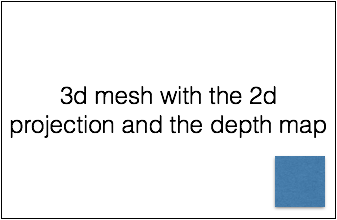
\includegraphics[width=0.7\textwidth]{figures/generative_fig.png}
\label{genfigure}
\caption{A 3D mesh $\M$ is expressed in terms of a ``sampling" 2D irregular mesh $\tilde{\M}$ and a depth scalar field $f$ over $\tilde{\M}$.}  
\end{figure}

In this work, we consider the variational autoencoder framework \cite{vae, vae2}. 
It considers a mixture model of the form 
\begin{equation}
\label{ban1}
p(\M) = \int p_\theta(\M ~|~h) p_0(h) dh~,
\end{equation}
where $h \in \R^S$ is a vector of latent variables. 
As observed by some authors \cite{ganvsvae}, 
mixture models such as (\ref{ban1}) when modeling natural images
suffer to recover high-frequency information. A possible 
explanation for that comes from the fact that variability due to 
geometric deformations is highly nonlinear in the pixel space, 
and is therefore hard to describe with additive mixtures using
unimodal likelihood terms $p_\theta( x ~|~h)$ \cite{superresjoan}. 
However, in surfaces, as described in Section \ref{stabsection}, 
geometric deformations are additive perturbations on the node 
coordinates, making mixture models an appealing choice.

%Variational Autoencoder framework. 
%We describe here the encoder and the decoder model. 
We thus consider a variational auto-encoder associated to model (\ref{ban1}), 
which optimizes the variational lower bound of the data log-likelihood:
\begin{equation}
\min_{\theta, \psi} \frac{1}{L} \sum_{l \leq L} - \E_{ h \sim q_\psi(h ~|~\M_l)} \log p_\theta( \M_l ~|~h) + D_{KL}( q_\psi( h~|~\M_l) ~||~p_0(h) )~.
\end{equation}
We thus need to specify a conditional generative model $p_\theta(\M ~|~h)$, 
a prior distribution $p_0(h)$ and a variational approximation to the posterior
$q_\psi( h ~|~ \M)$, where $\theta$ and $\psi$ denote respectively generative 
and variational trainable parameters.
Based on the height-field representation, we choose for simplicity a separable model of the form
$$p_\theta(\M ~|~h) =  p_\theta( f~|~h, \tilde{\M}) \cdot p(\tilde{\M}) ~,$$
where $\tilde{\M} \sim p(\tilde{\M})$ is a homogenous Poisson point process, 
and $f \sim p_\theta( f~|~h, \tilde{\M})$ is a Normal distribution with 
mean and isotropic covariance parameters given by a surface neural network:
$$p_\theta( f~|~h, \tilde{\M}) = {\cal N}( \mu(h, \tilde{\M}), \sigma^2(h, \tilde{\M}) {\bf 1})~,~\text{with } [ \mu(h, \tilde{\M}), \sigma^2(h, \tilde{\M})] = \Phi_D(\tilde{M}; h)~.$$
The generation step thus proceeds as follows.
we first sample a 2D mesh $\tilde{\M}$ independent of the latent variable $h$, 
and then sample a depth field over $\tilde{\M}$ conditioned on $h$ from the output
of a decoder network $\Phi_D(\tilde{M}; h)$.

Finally, the variational family $q_\psi$ is also a Normal distribution whose parameters 
are obtained from an encoder Surface Neural Network whose last layer is a global pooling that removes 
the spatial localization:
$$q_\psi( h~|~\M) = {\cal N}(\bar{\mu}, \bar{\sigma}^2 {\bf 1})~,~\text{ with }~ [\bar{\mu}, \bar{\sigma}] = \bar{\Phi}_D(\M)~.$$

Comment on the limitations.

Generalization to other Euler Characteristic is immediate. 




\section{Experiments}

\appendix

\section{The Dirac Operator}

spin transformations
conformal maps
quaternions.


\section{Further Numerical Experiments}


\section{Proof of Theorem \ref{stabtheo}}
 
 \subsection{Proof of (a)}
 We first show the result for the mapping $x \mapsto \rho \left( A x + B \Delta x \right)$, 
 corresponding to one layer of $\Phi_\Delta$. 
 By definition, the Laplacian $\Delta$ of $\M$ is 
 $$\Delta = \text{diag}(\bar{\ba})^{-1}( D - W)~,~$$
where $\bar{\ba}_j$ is one third of the total area of triangles incident to node $j$, 
and $W=(w_{i,j})$ contains the cotangent  weights \cite{laplacian_conv}.

From \cite{laplace_bound} we verify that 
\begin{eqnarray}
\label{ble4}
\| D - W \| &\leq& \sqrt{2} \max_{j} \left( d(j)^2 + \sum_{i \sim j} d(i) \right)^{1/2}  \\
&\leq& 2\sqrt{2} \sup_{i,j} w_{i,j} \sup_j S(j) \nonumber \\
&\leq& 2 \sqrt{2} \cot ( \alpha_{\text{min}} ) S_{\text{max}} ~, \nonumber
\end{eqnarray}
where $S(j)$ denotes the number of neighbors of node $j$, 
$\alpha_{\text{min}}$ is the smallest angle in the triangulation of $\M$ and $S_{\text{max}}$ the 
largest number of incident triangles. 
It results that 
$$\| \Delta \| \leq C \frac{\cot ( \alpha_{\text{min}} ) S_{\text{max}}}{\inf_j \bar{\ba}_j}:= L_\M~,$$
which depends uniquely on the mesh $\M$ and is finite for non-degenerate meshes. 
Moreover, since $\rho(\,\cdot \,)$ is non-expansive, we have
\begin{eqnarray}
\label{za1}
\left\| \rho \left( A x + B \Delta x \right) - \rho\left( A x' + B \Delta x' \right) \right \| & \leq & \| A( x - x') + B \Delta (x-x') \| \\ \nonumber
& \leq & (\| A \| + \| B \| L_\M ) \| x - x'\|~. 
\end{eqnarray}

By cascading (\ref{za1}) across the $K$ layers of the network, we obtain
\begin{equation*}
\| \Phi(\M; x) - \Phi(\M; x') \| \leq \left(\prod_{k \leq K} ( \| A_k \| + \| B_k \| L_\M) \right) \| x - x' \|~,
\end{equation*}
which proves (\ref{ya1}).

\subsection{Proof of (b)}

To establish (\ref{ya2}) we first observe that given three points $p, q, r \in \R^3$ forming any of the triangles of $\M$, 
\begin{eqnarray}
\| p - q \|^2 (1 - | \tau |_\infty)^2 &\leq \| \tau(p) - \tau(q) \|^2 \leq& \| p - q \|^2 (1 + | \tau |_\infty)^2 \label{za3} \\
\ba(p,q,r)^2 ( 1 - | \tau |_\infty C \alpha_{\text{min}}^{-1} - o(|\tau |_\infty^2) & \leq \ba(\tau(p), \tau(q), \tau(r) )^2 \leq & \ba(p,q,r)^2 ( 1 + | \tau |_\infty C \alpha_{\text{min}}^{-1} + o(|\tau |_\infty^2))~. \label{za4}  
\end{eqnarray}
Indeed, (\ref{za3}) is a direct consequence of the lower and upper Lipschitz constants of $\tau(u)$, which are bounded respectively by $1- | \tau|_\infty$ 
and $1 + | \tau|_\infty$. As for (\ref{za4}), we use the Heron formula 
$$\ba(p,q,r)^2 = s ( s - \| p - q \|)( s - \| p - r \|)( s - \| r - q \|)~,$$
with $s = \frac{1}{2}( \| p - q \| + \| p - r \| + \| r - q \|)$ being the half-perimeter.
By denoting $s_\tau$ the corresponding half-perimeter determined by the deformed points $\tau(p), \tau(q), \tau(r)$, 
we have that 
$$ s_\tau - \| \tau(p) - \tau(q) \| \leq s(1 + |\tau|_\infty) - \| p - q \| ( 1 - |\tau|_\infty) = s -  \| p - q \|  + |\tau|_\infty( s + \| p - q \|)~\text{and }$$
$$ s_\tau - \| \tau(p) - \tau(q) \| \geq s(1 - |\tau|_\infty) - \| p - q \| ( 1 + |\tau|_\infty) = s -  \| p - q \|  - |\tau|_\infty( s + \| p - q \|)~,$$
and similarly for the $\| r - q\|$ and $\|r - p \|$ terms. 
It results that
\begin{eqnarray*}
\ba(\tau(p),\tau(q),\tau(r))^2 &\geq& \ba(p,q,r)^2 \left[ 1 - | \tau|_\infty \left( 1 + \frac{s + \| p - q \|}{s - \| p -q \|} + \frac{s + \| p - q \|}{s - \| p -q \|} + \frac{s + \| p - q \|}{s - \| p -q \|} \right) - o( |\tau|^2 )\right ]  \\
&\geq & \ba(p,q,r)^2 \left[ 1 - C | \tau|_\infty \alpha_{\text{min}}^{-1}  - o( |\tau|^2) \right]~,
\end{eqnarray*}
and similarly 
$$\ba(\tau(p),\tau(q),\tau(r))^2  \leq \ba(p,q,r)^2 \left[ 1 + C | \tau|_\infty \alpha_{\text{min}}^{-1}  - o( |\tau|^2) \right] ~.$$

By noting that the cotangent Laplacian weights can be written (see Fig. ?) as
$$w_{i,j} = \frac{- \ell_{ij}^2 + \ell_{jk}^2 + \ell_{ik}^2 }{\ba(i,j,k)} + \frac{- \ell_{ij}^2 + \ell_{jh}^2 + \ell_{ih}^2 }{\ba(i,j,h)}~, $$
we have from the previous Bilipschitz bounds that
$$\tau( w_{i,j}) \leq w_{i,j} \left[ 1 - C | \tau|_\infty \alpha_{\text{min}}^{-1}\right]^{-1} + 2 | \tau|_\infty \left[ 1 - C | \tau|_\infty \alpha_{\text{min}}^{-1}\right]^{-1} \left( \frac{\ell_{ij}^2 + \ell_{jk}^2 + \ell_{ik}^2}{\ba(i,j,k)} + \frac{\ell_{ij}^2 + \ell_{jh}^2 + \ell_{ih}^2}{\ba(i,j,h)} \right)~,$$
$$\tau( w_{i,j}) \geq w_{i,j} \left[ 1 + C | \tau|_\infty \alpha_{\text{min}}^{-1}\right]^{-1} - 2 | \tau|_\infty \left[ 1 + C | \tau|_\infty \alpha_{\text{min}}^{-1}\right]^{-1} \left( \frac{\ell_{ij}^2 + \ell_{jk}^2 + \ell_{ik}^2}{\ba(i,j,k)} + \frac{\ell_{ij}^2 + \ell_{jh}^2 + \ell_{ih}^2}{\ba(i,j,h)} \right)~,$$
which proves that, up to second order terms, the cotangent weights are Lipschitz continuous to deformations. 

Finally, since the mesh Laplacian operator is constructed as $\text{diag}(\bar{\ba})^{-1} (D - W)$, 
with $\bar{\ba}_{i,i} = \frac{1}{3} \sum_{j,k; (i,j,k) \in F} \ba(i,j,k)$, and $D = \text{diag}( W {\bf 1})$,
let us show how to bound $\| \Delta - \tau(\Delta) \|$ from
\begin{equation}
\label{pep1}
\bar{\ba}_{i,i} ( 1 - \alpha_\M | \tau|_\infty - o( | \tau|^2) ) \leq \tau(\bar{\ba}_{i,i}) \leq \bar{\ba}_{i,i} ( 1 + \alpha_\M | \tau|_\infty + o( | \tau|^2) )
\end{equation} 
and
\begin{equation}
\label{pep2}
w_{i,j} ( 1 - \beta_\M | \tau|_\infty - o( | \tau|^2) ) \leq \tau(w_{i,j}) \leq w_{i,j} ( 1 + \beta_\M | \tau|_\infty + o( | \tau|^2) )~.
\end{equation} 
Using the fact that $\bar{\ba}$, $\tau(\bar{\ba})$ are diagonal, and using the spectral bound for $k \times m$ sparse matrices 
from \cite{splitting}, Lemma 5.12, 
$$\| Y \|^2 \leq \max_i \sum_{j ; \, Y_{i,j} \neq 0} |Y_{i,j}| \left( \sum_{r=1}^l | Y_{r,j}| \right)~, $$
the bounds (\ref{pep1}) and (\ref{pep2}) 
yield respectively 
\begin{eqnarray*}
\label{pep3}
 \tau(\bar{\ba}) &=& \bar{\ba} ( {\bf 1} + \epsilon_\tau)~,~\text{with } \| \epsilon_\tau \| = o( | \tau|_\infty)~,\text{and}  \\
 \tau( D - W) &=& D - W + \eta_\tau~,~\text{with } \| \eta_\tau \| = o ( | \tau|_\infty )~.
\end{eqnarray*}
%We note that the bound only depends on $N$, the size of the mesh, through the largest degree 
%of the mesh, which is bounded in regular meshes, and through the smallest angle $\alpha_{\min}$. 
It results that, up to second order terms, 
\begin{eqnarray*}
\| \Delta - \tau(\Delta) \| &=& \left \| \tau(\bar{\ba})^{-1} ( \tau(D) - \tau(W) ) - \bar{\ba}^{-1} ( D - W) \right\| \\
&=& \left \| \left( \bar{\ba} [{\bf 1} + \epsilon_\tau ] \right)^{-1} \left[ D - W + \eta_\tau \right] - \bar{\ba}^{-1} ( D - W) \right\| \\
&=& \left \| \left( {\bf 1} - \epsilon_\tau + o(|\tau|_\infty^2) \right) \bar{\ba}^{-1} ( D - W + \eta_\tau) - \bar{\ba}^{-1} ( D - W)  \right\| \\
&=& \left \| \epsilon_\tau \Delta + \bar{\ba}^{-1} \eta_\tau \right\| + o( | \tau |_\infty^2) \\ 
&=& o( | \tau|_\infty)~,
\end{eqnarray*}
which shows that the Laplacian is stable to deformations in operator norm. 
Finally, by denoting $\tilde{x}_\tau$ a layer of the deformed Laplacian network 
$$\tilde{x}_\tau = \rho( A x + B \tau(\Delta) x)~,$$
it follows that 
\begin{eqnarray}
\label{pep4}
\| \tilde{x} - \tilde{x}_\tau \| &\leq& \| B ( \Delta - \tau(\Delta) x \| \\
&\leq & C \| B \| | \tau|_\infty \|x \| ~.
\end{eqnarray}
Also, 
\begin{eqnarray*}
\| \tilde{x} - \tilde{x'}_\tau \| &\leq& \| A( x - x') + B ( \Delta x - \tau(\Delta) x') \| \\
&\leq & (\| A \| + \| B \| \| \Delta \|  )\| x - x'\|  + \| \Delta - \tau(\Delta) \| \| x\| \\
& \leq & \underbrace{(\| A \| + \| B \| \| \Delta \|  )}_{\delta_1}\| x - x'\|  + \underbrace{C | \tau |_\infty}_{\delta_2} \| x \|~, 
\end{eqnarray*}
and therefore, by plugging (\ref{pep4}) with $x' = \tilde{x}_\tau$, 
$K$ layers of the Laplacian network satisfy 
\begin{eqnarray*}
\| \Phi(x; \Delta) - \Phi(x; \tau(\Delta) \| &\leq& \left(\prod_{j \leq K-1} \delta_1(j)\right) \| \tilde{x} - \tilde{x}_\tau\| + \left(\sum_{j < K-1} \prod_{j' \leq j} \delta_1(j') \delta_2(j) \right)  | \tau \|_\infty \|x \| \\
&\leq & \left[C  \left(\prod_{j \leq K-1} \delta_1(j)\right)  \|B \| +  \left(\sum_{j < K-1} \prod_{j' \leq j} \delta_1(j') \delta_2(j) \right)  \right] | \tau |_\infty \|x \| ~. ~~~ \square~.
\end{eqnarray*}

%We conclude by observing that the proof can be reproduced if we replace the Laplacian operator by the Dirac operator, since it 
%is defined in terms of the matrix $\bar{\ba}^{-1}$ and $L_{i,j} = v_i - v_j$. We can thus apply the same stability arguments of lengths
%and 


\subsection{Proof of (c)}

This result is an immediate consequence of the consistency of the cotangent Laplacian to the Laplace-Beltrami operator on $S$ \cite{laplacian_convergence}:
\begin{theorem}[\cite{laplacian_convergence}, Thm 3.4] Let $\M$ be a compact polyhedral surface which is a normal graph over a smooth surface $S$ 
with distortion tensor $\mathcal{T}$, and let $\bar{\mathcal{T}} = (\det \mathcal{T})^{1/2} \mathcal{T}^{-1}$. 
If the normal field uniform distance $\| \bar{\mathcal{T}} - {\bf 1} \|_\infty \leq \epsilon$, then
\begin{equation}
\label{blabla1}
\| \Delta_\M - \Delta_S\| \leq \epsilon~.
\end{equation}
\end{theorem}

Thus, given two meshes $\M$, $\M'$ approximating a smooth surface $S$ in terms of uniform normal distance, 
and the corresponding irregular sampling $x$ and $x'$ of an underlying function $\bar{x} : S \to \R$, we have 
\begin{equation}
\label{blabla2}
\| \rho( A x + B \Delta_{\M} x) - \rho( A x' + B \Delta_{\M'} x') \| \leq \| A \| \| x - x' \| + \|B \| \| \Delta_\M x - \Delta_{\M'} x' \|~.
\end{equation}
Since $\M$ and $\M'$ both converge uniformly normally to $S$ and $\bar{x}$ is Lipschitz on $S$, it results 
that 
$$\| x - \bar{x} \| \leq \beta \epsilon~,\text{ and }~\| x' - \bar{x} \| \leq \beta \epsilon~,$$
thus $\| x - x' \| \leq 2 \beta \epsilon$. 
Moreover, thanks to (\ref{blabla1}) we have 
$$\| \Delta_{\M} - \Delta_{\M'} \| \leq 2 \epsilon~, $$
which from (\ref{blabla2}) results in 
\begin{eqnarray}
\| \rho( A x + B \Delta_{\M} x) - \rho( A x' + B \Delta_{\M'} x') \| &\leq& 2 \| A \| \beta \epsilon +  \\
&& + \| B \| \| \Delta_\M x - \Delta_{\M'} x + \Delta_{\M'} x - \Delta_{\M'} x'  \| \nonumber \\
&\leq & \epsilon \left( 2 \|A \| \beta + \| B \| \|x\| \right) +  \| B \| \| \Delta_{\M'}\|  \|x - x' \| \nonumber ~,
%&\leq & 2\epsilon \beta \left( \|A \|  + \| B \| \|x\|  +  \| B \| \| \Delta_{\M'}\| \right)~.
\end{eqnarray}
and therefore 
\begin{eqnarray*}
\| \Phi_\M(x) - \Phi_{\M'}(x') \| &\leq& \left(\prod_{k \leq K} \|B_k \| \| \Delta_{\M} \| \right) \| x - x'\| + \epsilon \left[\sum_{k \leq K} \left( 2 \|A_k \| \beta + \| B_k \| \|x\| \right)  \prod_{k' \leq k} \|B_{k'} \| \| \Delta_{\M} \| \right]~ \\
&\leq& \epsilon \left\{2 \beta  \left(\prod_{k \leq K} \|B_k \| \| \Delta_{\M} \| \right) + \left[\sum_{k \leq K} \left( 2 \|A_k \| \beta + \| B_k \| \|x\| \right)  \prod_{k' \leq k} \|B_{k'} \| \| \Delta_{\M} \| \right]  \right\}~.~~~\square~.
\end{eqnarray*}


\section{Proof of Corollary \ref{corocombine}}

$D_\tau S$ is linear: $D_\tau S = S + b(\tau)$, 
$\| \Delta b(\tau) \|$ small if $b(\tau)$ is smooth.  


\section{Proof of Theorem \ref{diractheo}}







\end{document}




